%!TEX root = thesis.tex
\chapter{Cryptographic Primitives}
Secure Compuation (SC) is the study of computing functions in a secure fashion. 
SC can be split into two cases: cases where there are two parties involved, referred to as two-party computation (2PC), and cases where there are three or more parties, referred to as multiparty computation (MPC).
This thesis will focus primarily on 2PC protocols, but many of the methods are applicable to MPC as well.

2PC protocols are complex cryptographic protocols that rely on a number of cryptographic primitives.
In order to understand 2PC, it is not crucial to understand how the cryptographic primitives work, but it is important to understand their inputs, outputs and security guarantees. 
This first chapter will give an overview of the cryptographic primitives used in 2PC protocols.

\section{A Brief Introduction to Cryptography} 
What does it mean for a cryptographic scheme to be secure? 
The goal of this section is to explain cryptographic security, starting at an intuitive level and moving outward. 
We do not present cryptographic security in a comprehensive fashion; rather, we explain cryptographic security with the goal of explaining 2PC protocols and their security.
For more information on cryptographic security, we encourage the reader to peruse \cite{katzlindelltextbook}. 

We define a few intuitive terms to get started.
A \textit{cryptographic scheme} is a series of instructions designed to perform a specific task. 
An \textit{adversary} is an algorithm that tries to \textit{break} the scheme. 
If an adversary \textit{breaks} a scheme, then the adversary has learned information about inputs to the scheme that they shouldn't. 

The goal of defining security in cryptography is to build a formal definition that matches real world needs and intuitions. 
A good starting place is to consider perfect security. 
A scheme is perfectly secure if no matter what the adversary does, they cannot break the scheme.
In particular, we imagine that the adversary has unlimited computational power, and they can still not break the scheme.

However, this is not the most useful way to think of security, because it makes it very difficult to make useful and fast schemes. 
We loosen the definition of security by saying that the adversary must run in polynomial time. 
This substantially reduces the possibilities of the adversary, but is also realistic. 
An algorithm that does not run in polynomial-time takes a substantial amount of time to run, given a sufficiently large input. 

It is also useful to be able to scale how secure a scheme is. 
A cryptographic scheme that was secure in the early 2000s probably should not be considered now. 
What was considered a reasonable adversary back then is simply different from adversaries now. 
As a concrete example, consider an giving an adversary the following problem: find the factors of $N$. 
The average computer today can solve the problem for a larger $N$ than the average computer a decade ago.

To model this idea, we introduce a \textit{security parameter}, denoted as $\lambda$.
A security parameter is a positive integer that represents how hard a scheme is to break. 
A larger security parameter should mean that the scheme is more difficult to break. 
More specifically, the security parameter is correlates to the input-size of the problem underlying the cryptographic scheme. 
For example, if the underlying problem is factoring large number $N$, then $N = \lambda$. 
As $N$ and $\lambda$ scale up, the factoring problem becomes more difficult and the scheme becomes hard to break. 

The following formalizes the previous discussion.
In order to reason about the security of cryptographic schemes, it is useful to think about breaking the scheme in terms a probability. 
To achieve this, we introduce a negligible function.
Intuitively, a negligible function is smaller than all polynomial functions. 
Formally, a negligible function is defined as follows:

\begin{definition}
\label{defn:negible}
A function $\mu : \NN \to \RR$ is negligible if for all positive polynomial $p(\cdot)$, there exists positive integer $N_p$ such that for all $x > N_p$, 
\begin{equation}
    |\mu(x)| < \frac{1}{p(x)}.
\end{equation}
\cite{goldreich}
\end{definition}

Examples of negligible functions include $2^{-n}$, $2^{- \sqrt{2}}$ and $n^{- \log n}$. 

To put a negligible function to use, say an adversary is attacking a cryptographic scheme that is equivalent to solving a problem $P$ with input-size $\lambda$ and $2^{\lambda}$ possible answers. 
Moreover, say that $P$ is known to be NP-hard such that there is no polynomial time algorithm to solve $P$. 
Then, the best that the adversary can do is to guess the answer to $P$.
Hence the probability that the adversary that finds the answer the $P$, or breaks the scheme, is 
\begin{align*}
Pr[\text{A correctly answers $P$}] & = {2^{- \lambda}}
\end{align*}
Since $2^{- \lambda}$ is a negligible function, we say that the adversary has a negligible probability of breaking the scheme. 

Real world - Ideal world?

We now introduce the idea of computational indistinguishability. 
Informally, two probability distributions are computationally indistinguishable if no polynomial-time algorithm can tell them apart. 
\al{TODO}
This is a useful idea because ...
For concreteness, imagine that ...

Formally, computational indistinguishability is:
\begin{definition}
\label{defn:computational-indistinguishability}
Let $\mathcal{X} = \{X_n\}_{n \in \NN}$ and $\mathcal{Y} = \{Y_n\}_{n \in \NN}$ be distribution ensembles.
$\mathcal{X}$ and $\mathcal{Y}$ are computationally indistinguishable, denoted $\mathcal{X} \compindist \mathcal{Y}$, if for all probabilistic polynomial-time algorithms $D$, there exists a negligible function $\mu$ such that:
\begin{equation}
	\al{Not right yet. page 277 in book}
    |Pr[D(1^n, x) = 1] - Pr[D(Y) = 1]| < \mu(n)
\end{equation}
\cite{lindell2009secure}.
\end{definition}


\section{Encryption}
\al{add in from google drive}
\begin{equation}
    \label{eqn:encryption}
    \begin{split}
        \Enc_k (pt) & = ct  \\
        \Dec_k(pt) = \EncInv_k(ct) & = pt
    \end{split}
\end{equation}
where $pt$ is the original message or the \emph{plaintext}, $ct$ is the encrypted message or the \emph{ciphertext}, and $k$ is the secret key.
For the algorithm to be effective, the secret key $k$ must be randomly sampled from $\{0,1\}^\lambda$, where $\lambda$ is the security parameter of our protocol.\footnote{The notion of randomness in cryptography is precisely defined, and in cases where $\lambda$ is large, it is sufficient for $k$ to be pseudorandom. Pseudorandomness is also precisely defined.}
\al{does footnote go before or after period? ShouldI have footnotes?}
If  $\lambda$ is increased, thereby increasing the size of the key, then the encryption algorithm becomes harder to break.
We will not go into details about how encryption algorithms are instantiated; we will merely treat them as algorithms which we can use at our leisure.

\begin{definition}
\al{Get crypto book and finish this}
We say that an encryption scheme is secure if:\footnote{Specifically, this is the definition of a chosen-plaintext-attack secure encryption scheme. There exists weaker and stronger definitions of security, but chosen-plaintext-attack security is frequently used for 2PC}

Define the following game:
What are the inputs?
\begin{enumerate}
\item Adversary picks two messages $m_0$ and $m_1$, and gives $m_0$ and $m_1$ to the sender. 
\item The sender samples $k \gets \{0,1\}^{\lambda}$ and $b \gets \{0,1\}$. The sender gives $m_b$ to the adversary. 
\item The adversary may spend a polynomial amount of time doing computation. Eventually, the output $b'$, their guess as to which message they received.
\end{enumerate}
\end{definition}
% END WORK HERE

It is useful for 2PC to define a specific type of symmetric-key encryption algorithm called a \textit{dual-key cipher} (DKC) \cite{bellare2012foundations}.
A DKC requires two keys to encrypt and decrypt the message, in contrast to classic encryption which only requires one.
It is easy to instantiate a DKC if one has a secure encryption scheme: let $k_0$ and $k_1$ be two keys and instantiate the DKC as follows:
\begin{equation}
    \begin{split}
        \EncDKC_{k_0, k_1}(pt) = \Enc_{k_1} ( \Enc_{k_0} ( pt )) \\
        \EncDKCInv_{k_0, k_1}(ct) = \EncInv_{k_0} ( \EncInv_{k_1} ( ct )) 
    \end{split}
\end{equation}
This construction of a DKC is slow, and there are many faster methods for instantiating DKCS.
For more information, see \cite{bellare2012foundations}.

\section{Boolean Circuit} 
A function in a 2PC protocol is represented as a boolean circuit.
A boolean circuit takes as input $x \in \{0,1\}^n$, performs a series of small operations on the inputs, and outputs $y \in \{0,1\}^m$.  
You may have encountered circuits and logical operators in another context, where the inputs and outputs were True and False.
For our usage, True will correspond to the value $1$, and False will corresond to the value $0$. 

The small operations done inside of a circuit are performed by a \emph{gate}.
A gate is composed of three wires: two input wires and one output wire, where a \emph{wire} can have a value either $0$ or $1$.
A gate performs a simpler operation on the two inputs, resulting in a single output bit.
Table \ref{tab:xor} gives the mapping of an XOR gate.

\begin{table}[h]
\label{tab:xor}
\centering
\begin{tabular}{ | l | c || r |}
\hline
x & y & xor(x,y) \\ \hline
1 & 1 & 0 \\ \hline
1 & 0 & 1 \\ \hline
0 & 1 & 1 \\ \hline
0 & 0 & 0 \\ \hline
\end{tabular}
\caption{The mapping of an XOR gate.}
\end{table}

A circuit is a combination of gates that are stringed together.
It turns out that circuits are quite powerful: in fact, a circuit composed only of AND gates, XOR gates and NOT gates can compute any function or algorithm \cite{Goldreich}.
In other words, if there's some algorithm that can do it, then there is some circuit that can do it as well.
Figure \ref{fig:less_than_circuit} shows the circuit representation of the less than function, $f$ as specified in equation \ref{eqn:less_than}.

\begin{figure}[h]
    \centering
    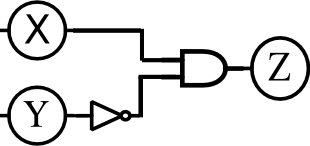
\includegraphics[scale=0.75]{images/drawing.png}
    \label{fig:less_than_circuit}
    \caption{A circuit that computes the less or equal to function, equivalent to the less than function for input of two one-bit values.\al{define symbols and google circuit diagrams latex / tree diagrams}}
\end{figure}

\begin{table}[h]
\label{tab:less_than}
\centering
\begin{tabular}{ | l | c || r |}
\hline
x & y & $x < y$ \\ \hline
0 & 0 & 0 \\ \hline
0 & 1 & 1 \\ \hline
1 & 0 & 0 \\ \hline
1 & 1 & 0 \\ \hline
\end{tabular}
\caption{The truth table of the less than circuit.}
\end{table}

\section{Oblivious Transfer}
\al{more sources here - get from CompGC paper}
\al{Give a nice metaphor of using OT - what happens. Don't need to give the protocol}
Oblivious Transfer (OT) is a two-party protocol where one party (sender) has two inputs, $m_0$ and $m_1$, and the other party (receiver) has a bit $b \in \{0,1\}$. 
OT enables the receiver to acquire $m_b$ from the sender without revealing which message is received, i.e., the value of $b$.
Moreover, the receiver learns nothing about the message that isn't received, i.e. anything about $m_{1-b}$.

The protocol relies on the DDH assumption.\footnote{The Decisional Diffie-Hellman (DDH) assumption is a computational hardness assumption involving discrete logarithms in cyclic groups. For more information, see \cite{Boneh1998}.}


